\documentclass[twocolumn,tikz]{handout}
\usepackage{amsmath}
\usepackage{physics}
\usepackage[outline]{contour}
\usepackage[latin1]{inputenc}
\usepackage[T1]{fontenc}
\usepackage[pdftex]{graphicx}
%\usepackage{color}
\usepackage{hyperref}
\usepackage{dsfont}
\usepackage[dvipsnames]{xcolor}
\usepackage{footmisc}
\usepackage{tikz}
\usepackage{pgfplots}
\usepgfplotslibrary{fillbetween}
\usetikzlibrary{decorations.markings}
\usetikzlibrary{patterns}
\usetikzlibrary{positioning}

\usetikzlibrary{angles,quotes} % for pic
\usetikzlibrary{bending} % for arrow head angle
\contourlength{1.0pt}
\usetikzlibrary{3d}

\tikzset{>=latex} % for LaTeX arrow head
\colorlet{myblue}{blue!65!black}
\colorlet{mydarkblue}{blue!50!black} \colorlet{myred}{red!65!black}
\colorlet{mydarkred}{red!40!black} \colorlet{veccol}{green!70!black}
\colorlet{vcol}{green!70!black} \colorlet{xcol}{blue!85!black}
\tikzstyle{vector}=[->,very thick,xcol,line cap=round]
\tikzstyle{xline}=[myblue,very thick] \tikzstyle{yzp}=[canvas is zy
plane at x=0] \tikzstyle{xzp}=[canvas is xz plane at y=0]
\tikzstyle{xyp}=[canvas is xy plane at z=0]
\def\tick#1#2{\draw[thick] (#1) ++ (#2:0.12) --++ (#2-180:0.24)}
\def\N{100}

\pgfplotsset{width=7cm,compat=1.3}

\SetInstructor{José Luis Álvarez Pérez} \SetCourseTitle{TFG}
\SetHandoutTitle{Transformación entre puntos del campo
cercano.\vspace{1ex}}
\SetSemester{Aitor Ingelmo} %\SetDueDate{28 Febrero}

\begin{document}

\maketitleinst

\section{El desarrollo modal del campo}
Vamos a empezar por justificar la ecuación (12-73) del libro de
Balanis \textit{Antenna Analysis and Design}, que para nosotros va a
ser la ecuación \eqref{eq-fourier2a} de estas notas. Partimos de
considerar un campo eléctrico de frecuencia dada $\omega$
\begin{equation}
\vec{\tilde{E}}(\vec{r},t)=\vec{E}(\vec{r})\,e^{j\omega t}
\label{eq-Ert}
\end{equation}
La ecuación de ondas para el campo eléctrico tiene esta forma:
\begin{equation}
\nabla^{2} \vec{\tilde{E}}(\vec{r},t)=\frac{1}{c}\frac{\partial^{2}
\vec{\tilde{E}}(\vec{r},t)}{\partial t^{2}}
\label{eq-we}
\end{equation}
lo que, evidentemente, lleva a la denominada ecuación de Helmholtz:
\begin{subequations}
\begin{align}
(\nabla^{2}+k^{2})\vec{E}(\vec{r})&=0\nonumber
\\
k&=\frac{\omega}{c}
\label{eq-He}
\end{align}
\end{subequations}

Suponemos ahora que tenemos un campo $\vec{\tilde{E}}(\vec{r})$ que
estamos en condiciones de medir en un plano, que suponemos que está
colocado de manera paralela al eje $XY$ y en una posición $z=z_{m}$.
La función bidimensional $\vec{E}(x,y,z=z_{m})$ se puede representar
mediante una integral de Fourier:
\begin{equation}
\vec{E}(x,y,z=z_{m})=\int_{-\infty}^{\infty}\int_{-\infty}^{\infty}\vec{\hat{E}}(k_{x},k_{y},z=z_{m})
\,e^{-j (k_{x} x+k_{y} y)} dk_{x} dk_{y}
\label{eq-fourier1}
\end{equation}
Si introducimos esta expresión en \eqref{eq-He} y devolvemos la
generalidad a la coordenada $z$ más allá de ser, como hasta ahora,
un punto de medida $z_{m}$ , obtenemos lo siguiente
\begin{multline}
\left(\nabla^{2}+k^{2}\right)\left(\int_{-\infty}^{\infty}\int_{-\infty}^{\infty}\vec{\hat{E}}(k_{x},k_{y},z)
\,e^{-j (k_{x} x+k_{y} y)} dk_{x}
dk_{y}\right)=\\
\int_{-\infty}^{\infty}\int_{-\infty}^{\infty}\left(\nabla^{2}+k^{2}\right)\left[\vec{\hat{E}}(k_{x},k_{y},z)
\,e^{-j (k_{x} x+k_{y} y)}\right] dk_{x} dk_{y}=0
\label{eq-fourier1andHe}
\end{multline}
Operando el Laplaciano, obtenemos
\begin{equation}
\int_{-\infty}^{\infty}\int_{-\infty}^{\infty}\left[\left(-k_{x}^{2}-k_{y}^{2}+k^{2}\right)+\frac{\partial^{2}}{\partial
z^{2}}\right]\left[\vec{\hat{E}}(k_{x},k_{y},z) \,e^{-j (k_{x}
x+k_{y} y)}\right] dk_{x} dk_{y}=0.
\label{eq-fourier1andHe2}
\end{equation}
Dado que esta igualdad se verifica para todo valor de $x$ e $y$, el
integrando ha de ser nulo:
\begin{equation}
\frac{\partial^{2}}{\partial
z^{2}}\vec{\hat{E}}(k_{x},k_{y},z)+w^{2}\vec{\hat{E}}(k_{x},k_{y},z)=0
\label{eq-He2}
\end{equation}
con

\begin{equation}
w^{2}=k^{2}-k_{x}^{2}-k_{y}^{2}.
\end{equation}

La solución de \eqref{eq-He2} viene dada, en general, por la
siguiente expresión

\begin{equation}
\vec{\hat{E}}(k_{x},k_{y},z)=\vec{\mathcal{E}^{+}}(k_{x},k_{y})\,e^{-j
w z}+\vec{\mathcal{E}^{-}}(k_{x},k_{y})\,e^{j w z}
\label{eq-eplus}
\end{equation}

donde $\vec{\mathcal{E}^{+}}(k_{x},k_{y})\,e^{-j w z}$ representa
una onda que se propaga en la dirección creciente de la $z$ mientras
que $\vec{\mathcal{E}^{-}}(k_{x},k_{y})\,e^{j w z}$ lo hace en la
dirección decreciente de la $z$. Para nuestro caso, solamente
consideramos la solución que contiene la
$\vec{\mathcal{E}^{+}}(k_{x},k_{y})\,e^{-j w z}$. Eso nos lleva a la
siguiente expresión para la ecuación \eqref{eq-fourier1}, que es la
ecuación (12-73) del libro de Balanis
\begin{equation}
\vec{E}(x,y,z)=\int_{-\infty}^{\infty}\int_{-\infty}^{\infty}\vec{\mathcal{E}^{+}}(k_{x},k_{y})
\,e^{-j (k_{x} x+k_{y} y+w  z)} dk_{x} dk_{y}
\label{eq-fourier2a}
\end{equation}

De todo esto extraeremos en la siguiente sección los pasos de un
algoritmo que nos permitirá calcular el campo eléctrico en una
posición $z$ cualquiera, en la que se supone que lo conocemos, y que
no tiene por qué ser la de salida de la onda, es decir, no tiene por
qué corresponderse al plano radiante de una antena, sino que puede
ser cualquier plano colocado delante de la misma. Estamos hablando
por tanto de un algoritmo para calcular el campo en un plano
geométrico dado por una $z$ concreta a partir de los valores en otro
plano del campo cercano. ¿Por qué lo denominamos ``cercano''? ¿Dónde
hemos introducido la hipótesis de que sea ``cercano''? En ningún
sitio. Precisamente, la hipótesis será después la de considerar el
``campo lejano'' como aquel para el que $z$ es suficientemente
grande, y en el que haremos algunas simplificaciones, propias de una
distancia grande a la fuente de la onda. Para contraponer ese campo
lejano al caso en el que no añadimos hipótesis simplificadoras
basadas en un valor de $z$ grande, utilizamos el adjetivo
``cercano'' como antónimo de ``lejano'', queriendo decir que no se
pueden hacer esas hipótesis derivadas de una $z$ grande.

\begin{figure}
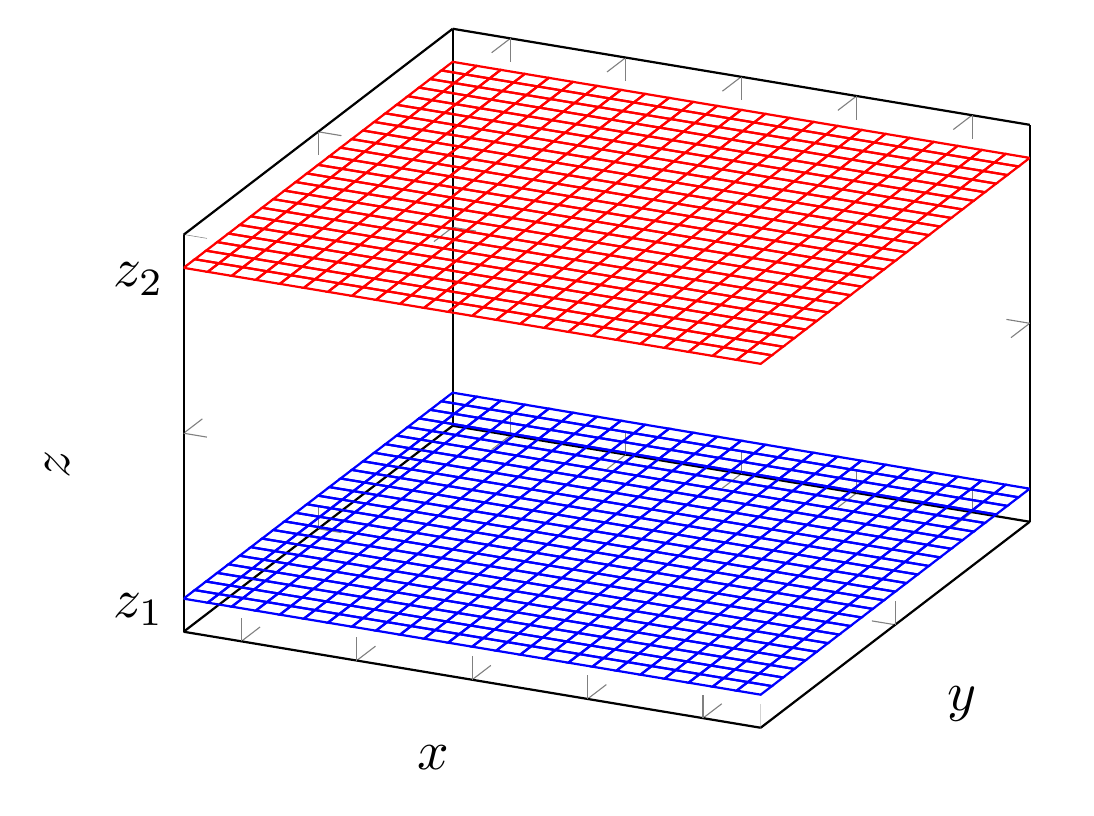
\begin{tikzpicture}[scale=2.0]
        \begin{axis}[
        xticklabels={,,},
        yticklabels={,,},
        zticklabels={$z_{2}$,'',$z_{1}$,,$z_{2}$},
        zlabel=$z$,
        xlabel=$x$,
        ylabel=$y$
        ]
            \addplot3[mesh] {5};
            \addplot3[mesh] {7};
        \end{axis}
\end{tikzpicture}
\caption{Se representan dos planos: sobre el plano azul hemos
realizado las medidas del valor del campo en todos los puntos que
son nodos de la rejilla y en el plano rojo se pretende inferir el
campo a partir de las medidas en el plano azul. La separación entre
nodos es de $\Delta x$ en la dirección $x$ y de $\Delta y$ en la
dirección $y$}
\end{figure}


\section{Algoritmo para transformar el valor del campo cercano en un
plano $z=z_{1}$ en el campo cercano en otro plano $z=z_{2}$}

Los pasos serían los siguientes:
\begin{itemize}
\item Estimamos los modos dados por la función
$\vec{\hat{E}}(k_{x},k_{y},z=z_{1})$. Para ello hay que partir de la
ecuación \eqref{eq-fourier1} e invertirla. En principio, la ecuación
inversa\footnote{En realidad, \eqref{eq-fourier2} tiene la forma de
la transformada de Fourier directa de $\vec{E}(x,y,z=z_{1})$ como
función de $x$ e $y$, mientras que la ecuación \eqref{eq-fourier1}
es formalmente la transformada inversa} sería
\begin{equation}
\vec{\hat{E}}(k_{x},k_{y},z=z_{1})=\frac{1}{(2\pi)^{2}}\int_{-\infty}^{\infty}\int_{-\infty}^{\infty}\vec{E}(x,y,z=z_{1})
\,e^{j (k_{x} x+k_{y} y)} dx dy.
\label{eq-fourier2}
\end{equation}
Las medidas de las que partimos no son continuas, sino que conocemos
el campo $\vec{E}(x,y,z=z_{1})$ en un conjunto de puntos
$(x,y)=(x_{n_{x}},y_{n_{y}})$ con $n_{x}=0,1,2,\ldots,N_{x}-1$ y
$n_{y}=0,1,2,\ldots,N_{y}-1$. Eso nos lleva a discretizar tanto
\eqref{eq-fourier1} como \eqref{eq-fourier2} de la siguiente manera:
empezamos por la ecuación \eqref{eq-fourier2}, que es la que nos
permite hallar los modos $\vec{\hat{E}}(k_{x},k_{y},z=z_{1})$

\begin{equation}
\vec{\hat{E}}(k_{x},k_{y},z=z_{1})=\frac{1}{(2\pi)^{2}}\Delta x
\Delta y
\sum_{n_{x}=0}^{N_{x}-1}\sum_{n_{y}=0}^{N_{y}-1}\vec{E}(x=n_{x}\Delta
x,n_{y} \Delta y,z=z_{1}) \,e^{j (k_{x} n_{x} \Delta x+k_{y} n_{y}
\Delta y)}
\label{eq-fourier3}
\end{equation}

donde $\Delta x=\frac{L_{x}}{N_{x}-1}$ y $\Delta
y=\frac{L_{y}}{N_{y}-1}$ con $L_{x}$ y $L_{y}$ como las dimensiones
de la apertura\footnote{Hay que tener en cuenta que la observación
del campo la vamos a realizar, no en un plano infinito, como parece
requerir la ecuación \eqref{eq-fourier2}, sino en una ``apertura''
finita.}. Con esta ecuación podemos estimar los modos para
cualesquier valores de $k_{x}$ y $k_{y}$, que podríamos utilizar
luego para calcular \eqref{eq-fourier1}. Parece, por tanto
conveniente utilizar el mayor número de valores posibles y construir
una ``malla'' de puntos $(k_{x},k_{y})$ mucho mayor potencialmente
que la de puntos en $(x,y)$, donde hemos visto que tenemos
$N_{x}\times N_{y}$ puntos. Este razonamiento tiene dos errores: no
tiene en cuenta el teorema del muestreo ni conecta con el
conveniente algoritmo de la Fast Fourier Transform (FFT). No vamos a
entrar en todo el detalle del primero, y basta decir que no por
tomar valores de $(k_{x},k_{y})$ vamos a tener una mejor descripción
de $\vec{E}(x,y,z)$ ya que hay un nivel de información máximo
asociado al muestreado en $(x,y)$. La FFT y su inversa están
diseñadas para tener esto en cuenta. Vamos a ponerlas a ambas como
sigue
\begin{equation}
\vec{\hat{E}}_{m_{x},m_{y}}=\frac{1}{N_{x} N_{y}}
\sum_{n_{x}=0}^{N_{x}-1}\sum_{n_{y}=0}^{N_{y}-1}
\vec{E}(x=n_{x}\Delta x,n_{y} \Delta y,z=z_{1}) \,e^{j 2\pi
\frac{m_{x} n_{x}}{N_{x}}}\,e^{j 2\pi \frac{m_{y} n_{y}}{N_{y}}}
\label{eq-fft1}
\end{equation}
para la FFT y
\begin{equation}
\vec{E}_{n_{x},n_{y}}=
\sum_{n_{x}=0}^{N_{x}-1}\sum_{n_{y}=0}^{N_{y}-1}
\vec{\hat{E}}_{m_{x},m_{y}} \,e^{-j 2\pi \frac{m_{x}
n_{x}}{N_{x}}}\,e^{-j 2\pi \frac{m_{y} n_{y}}{N_{y}}}
\label{eq-ifft1}
\end{equation}
para la IFFT (Inverse Fourier Transform). Podemos comparar ahora las
ecuaciones \eqref{eq-fft1} y \eqref{eq-fourier3} y vemos que, para
poder aprovechar la herramienta que nos brinda la FFT -y que,
recordemos, lleva de serie el teorema de muestreo-, tenemos que
hacer las siguientes identificaciones:
\begin{subequations}
\begin{align}
k_{x}&= m_{x}\Delta k_{x}
\\
k_{y}&= m_{y}\Delta k_{y}
\\
\Delta x \Delta k_{x}&=\frac{2\pi}{N_{x}}
\\
\Delta y \Delta k_{y}&=\frac{2\pi}{N_{y}}.
\end{align}
\end{subequations}
Vemos que las dos últimas igualdades, que son de obligado
cumplimiento si queremos ver la ecuación \eqref{eq-fourier3} como
una FFT, nos permiten definir los valores de $\Delta k_{x}$ y
$\Delta k_{y}$\footnote{Los de $\Delta x$ y $\Delta y$ están
definidos por nuestro muestreado del campo en el plano bajo
análisis, pero los de $\Delta k_{x}$ y $\Delta k_{y}$ aún no lo
estaban.} mediante
\begin{align}
\Delta k_{x}&=\frac{2\pi}{\Delta x N_{x}}
\\
\Delta k_{y}&=\frac{2\pi}{\Delta y N_{y}}
\end{align}

Lo que nos queda ahora es que la relación entre la
$\vec{\hat{E}}_{m_{x},m_{y}}$ de la ecuación \eqref{eq-fft1} y la
$\vec{\hat{E}}(k_{x},k_{y},z=z_{1})$ de la ecuación
\eqref{eq-fourier3} es la siguiente:
\begin{equation}
\vec{\hat{E}}(k_{x}=m_{x} \Delta k_{x},k_{y}=m_{y} \Delta
k_{y},z=z_{1})=\frac{L_{x}\,L_{y}}{(2\pi)^{2}}\frac{N_{x}}{N_{x}-1}\frac{N_{y}}{N_{y}-1}
\vec{\hat{E}}_{m_{x},m_{y}}
\end{equation}
donde, computacionalmente, usamos
\begin{equation}
\vec{\hat{E}}_{m_{x},m_{y}}=\mbox{FFT}\{\vec{E}(x=n_{x}\Delta
x,n_{y} \Delta y,z=z_{1})\}.
\end{equation}
Con esto hemos calculado los modos $\vec{\hat{E}}(k_{x}=m_{x} \Delta
k_{x},k_{y}=m_{y} \Delta k_{y},z=z_{1})$.

\item Se trata ahora de utilizar la ecuación \eqref{eq-fourier2a}
(la pondremos realmente como \eqref{eq-fourier1} con
\eqref{eq-eplus} y $\vec{\mathcal{E}^{-}}=0$, para ir más despacio,
pero es \eqref{eq-fourier2a} lo que usamos) para calcular el campo
en los puntos de otro plano $z=z_{2}$. Pero hemos dicho que vamos a
utilizar la pareja FFT-IFFT. 

Eso significa que, ahora, vamos a
discretizar la ecuación \eqref{eq-fourier2a} para que tome la forma
de la IFFT en \eqref{eq-ifft1}.

Eso lo conseguimos poniendo la
primera como
\begin{multline}
\vec{E}(x=n_{x}\Delta x,n_{y} \Delta y,z=z_{2})=\\
\Delta k_{x}
\Delta k_{y} \sum_{m_{x}=0}^{N_{x}-1}\sum_{m_{y}=0}^{N_{y}-1}
\vec{\hat{E}}(k_{x}=m_{x}\Delta k_{x},k_{y}=m_{y} \Delta
k_{y},z=z_{2}) \,e^{-j (n_{x} m_{x} \Delta x \Delta k_{x} +n_{y}
m_{y} \Delta x \Delta k_{x})}
\end{multline}
Gracias a la ecuación \eqref{eq-eplus} con
$\vec{\mathcal{E}^{-}}(k_{x},k_{y})=0$, podemos poner
\begin{equation}
\vec{\hat{E}}(k_{x},k_{y},z_{1})=\vec{\mathcal{E}^{+}}(k_{x},k_{y})\,e^{-j
w z_{1}}
\end{equation}
de donde despejamos la $\vec{\mathcal{E}^{+}}(k_{x},k_{y})$
\begin{equation}
\vec{\mathcal{E}^{+}}(k_{x},k_{y})=\vec{\hat{E}}(k_{x},k_{y},z_{1})\,e^{j
w z_{1}}
\end{equation}

y utilizamos ahora este valor en \eqref{eq-eplus} pero esta vez para
$z=z_{2}$ y los valores de las $k_{x}$ y $k_{y}$ correspondientes a
nuestro muestreo

\begin{align}
\vec{\hat{E}}(k_{x}=m_{x}\Delta k_{x},k_{y}=m_{y} \Delta
k_{y},z=z_{2})&=\vec{\mathcal{E}^{+}}(k_{x},k_{y})\,e^{-j w
z_{2}}=\nonumber
\\
\vec{\hat{E}}(k_{x}&=m_{x}\Delta k_{x},k_{y}=m_{y} \Delta
k_{y},z=z_{1})\,e^{-j w (z_{2}-z_{1})}
\end{align}
%\begin{equation}
%\vec{\hat{E}}(k_{x}=m_{x}\Delta k_{x},k_{y}=m_{y} \Delta
%k_{y},z=z_{2})=\vec{\hat{E}}(k_{x}=m_{x}\Delta k_{x},k_{y}=m_{y}
%\Delta k_{y},z=z_{1})\,e^{-j w (z_{2}-z_{1})}
%\end{equation}

De ahí obtenemos el campo en este otro plano $z=z_{2}$ mediante
\begin{equation}
\vec{E}(x=n_{x}\Delta x,n_{y} \Delta y,z=z_{2})=\Delta k_{x} \Delta
k_{y}\,\mbox{IFFT}\{\vec{\hat{E}}(k_{x}=m_{x}\Delta
k_{x},k_{y}=m_{y} \Delta k_{y},z=z_{2})\}.
\end{equation}


\end{itemize}

Advertencias:
\begin{enumerate}
\item Como el campo es vectorial, hay que aplicar separadamente este
algoritmo a todas las componentes.
\item Por supuesto, podemos trabajar con $\Delta x=\Delta y$
\item Los dos planos y las dos rejillas de medidas tienen que tener las mismas
dimensiones pero pueden ser subdominios de áreas mayores en las
cuales, por lo que sea, eliminamos ciertos márgenes. Eso ocurre en
el caso de trabajar con medidas simuladas sobre espacios esféricos,
donde los cortes con $z$'s dados no son iguales: nos quedamos con
los subdominios de iguales dimensiones.
\end{enumerate}

\end{document}
